\chapter{Programming in Natural Language} \label{chapter: Programming in Natural Language}
\section{Introduction}
Programming languages are textual, and so require a keyboard in order to edit programs. Standard on-screen keyboards are inconvenient for texting, let alone for programming. In addition, they take almost one-third of the screen which makes the small screen even smaller. In order to avoid using the inconvenient on-screen keyboard or an external device, we suggest to program by voice. Voice dictation is based on a common set of templates; these templates are individually customizable so that each developer can use the idioms that are most convenient for him or her.

We describe the idea of programming in natural language by writing requirements in order to bridge the gap between the code that the programmer wants to write and a code that is written on the screen. We claim that natural language can serve as the main tool for programming. We do not claim that it is the only tool, the programmer may use other gestures such as touch, on-screen keyboard, or external devices when needed 
\section{Configuration}
We suggest that every programmer will dictate in the most convenient way for him or her. Every one of us has a different way of describing the things that s/he wants to say. it is the same with code dictation.

For example, take the Java loop in \autoref{fig17}. We would dictate it character by character: "for, open parenthesis, int, space" etc. This is inconvenient and cumbersome. Instead, we would like to forget about the syntax and just describe what is needed. One way to say it is: "for i from zero to n". But another programmer may prefer to say "repeat n times" to describe the same loop.

We don't just dictate code from top to bottom; we also need to edit existing code and navigate to specific places in the code. Navigation depends on the context of what is shown on the screen and on the surrounding code. For example, if the screen contains only one loop, I can say "Go to the loop". Or I could say "Rename the index of the first loop to j" to navigate to the first loop on the screen and change its index variable. This demonstrates that templates used for dictation have named parts, and I can refer to these parts when I issue editing or navigation commands.
\begin{figure}[H]
	\begin{lstlisting}
	for(int i = 0; i < n; i++)
	\end{lstlisting}
	\caption{A simple for loop}
	\label{fig17}
\end{figure}
\section{Natural Language Processing}
In order to process dictation, we suggest a two-phase process: converting speech to text, and understanding the context of the text. We use a speech to text engine for the speech conversion and context free grammar to understand the context.
\subsection{Speech To Text Engines}
We found several speech-to-text engines that we can use for our solution: Nuance Dragon \citet{Nuance14} is a software developer kit (SDK) used by developers and integrators to add speech recognition capabilities into in-house and commercial applications or workflow applications. This toolkit, which enables everything from free-text dictation to command and control functionality, can be deployed as part of a server or client-based solution; Kaldi \citet{PoveyASRU2011} is a toolkit for speech recognition written in C++ and licensed under the Apache License v2.0. Kaldi is intended for use by speech recognition researchers. Google Speech Server V2 \citet{google15} is an online free speech-to-text engine which runs on a server, used primarily by researchers. We decided to use Google Speech Server V2 because it is free and easy to use. There are many more speech-to-text engines, but we decided to concentrate on the most well-known so Google Speech is the one that we choose to use.
\subsection{Context Free Grammar}
A context-free grammar (CFG) is a tuple $ G=(T,N,S,R) $, where $ T $ is the finite set of  terminals of the language, $ N $ is the set of non-terminals that represent phrases in a sentence, $ S \in N $ is the start variable used to represent a full sentence in the language. $ R $ is the set of production rules of the form $ N \rightarrow (N \bigcup T)* $.
\subsubsection{Extended Backus Naur Form}
Extended Backus Naur Form is a notation for formally describing syntax for how to write entities in language. The meta-language is based on a suggestion by Niklaus Wirth (Wirth, 1977) that is based on the Backus-Naur Form and that contains the most common extensions, i.e:
\begin{itemize}
	\item Terminal symbols of the language are quoted so that any character,
	including one used in Extended BNF, can be defined as a terminal symbol of
	the language being defined.
	\item $ [ $ and $ ] $ indicate optional symbols.
	\item $ \{ $ and $ \} $ indicate repetition.
	\item Each rule has an explicit final character so that there is never any
	ambiguity about where a rule ends.
	\item Brackets group items together. It is an obvious convenience to use ( and ) in their ordinary mathematical sense.
\end{itemize}
\subsection{Dictation Parser} \label{subsec: Dictation Parser}
We use EBNF to create a set of rules that will validate commands that the programmer dictates. This set of rules can be extended easily by every user to understand EBNF. We use IEEE\\IEC EBNF \cite{IEEEBNF1996} as our main reference to learn how to use EBNF. In \cite[pages 51-86]{Michal2009} Michal Gordon and David Harel claim that formal structured natural language requirements can serve as the means and the end to programming the behavior of reactive system using fully executable languages such as live sequence charts (LSC). We adopt this approach and use it to create a set of rules to process user dictation.

\subsubsection{Grammar Construction}
We now show how our grammar translates controlled natural language. Since we allow a CFG, we can increment the grammar with additional rules that allow various ways of generating similar constructs. We can thus increase the set of accepted specifications by augmenting the grammar. However, ambiguity may grow as the grammar grows which would require the user to explicitly disambiguate his intentions in too many cases for the process to be friendly. We shall describe how basic commands such as: creation, navigation, and modification are parsed. The \textit{Dictation Parser} tries to build a parse tree for every dictation that it receives. A valid dictation is one for which the \textit{Diction Parser} succeeded to create a parse tree. A number of advanced ideas are not yet supported in the current implementation. Nevertheless, the current grammar allows implementing fully executable systems, and has been tested, among other examples, on the \textit{LinkList} Example, and on the \textit{Command Pattern} Example, see \ref{subsection: Grammar Testing}.

The set of rules is divided into four main layers in the Parser layer: \textit{Top}, \textit{Categories}, \textit{Forms of Expressions}, and \textit{Common}. The \textit{Top} layer contains rules that have access to all categories. The \textit{Categories} layer contains sub-sections that is divided into different categories. For example, the \textit{Creation} sub-section contains all rules that deal with creation. The \textit{Common} layer knows nothing about any category, it contains all the necessary information for all actions. The \textit{Forms of Expressions} layer contains all all possible forms of expressing any command. For example, there are several options to pronounce that you want to return something from a method, you may say: "that returns", "returns", "return" and more. The \textit{Top} layer and the \textit{Categories} layer have access to the \textit{Common} layer and to \textit{Forms of Expressions} layers. The \textit{Common} layer has an access to the \textit{Forms of expressions} layer. \autoref{fig21} shows how rules are divided into layers and sub-categories. Note that this division has no effect on the action of rules. Its function is only to understand the set of rules better.

We now shall explain every sub-category inside the \textit{Categories} layer. \textit{Creation} contains all rules that parse any creation dictation. For example, "Create a new class". \textit{Navigation} contains all rules that parse any navigation dictation. For example, "Go to class person". \textit{Modification} contains all rules that parse any modification dictation.

We now discuss two dictations that have the same meaning but are expressed differently. It is important to Deverywhere to allow programmers to dictate code in their preferred way. Let’s assume that the programmer created a class \textit{Car} and now he wants to create an inner class \textit{Wheel}. One way to say it is \textit{"create a static public class named wheel inside class car"}. \autoref{fig18} presents the parse tree that is generated for this dictation. This dictation will lead to creating a new static class called \textit{Wheel} inside a class that is called \textit{Car}.   

\begin{figure}[H]
	\centering
	\includegraphics[scale=0.4]{"./fig/Parse Tree create a static public class named wheel inside class car"}
	\caption{The parse tree for the sentence "create a static public class named wheel inside class car".}
	\label{fig18}
\end{figure}

Another way to say it is \textit{"create an inner class wheel"}. In this case, the class that will be created won't be static and the cursor of the IDE shall be placed inside class \textit{Car}, otherwise the class \textit{Wheel} won't be created inside class \textit{Car}. \autoref{fig19} presents the parse tree that is generated for this dictation. This dictation will lead to creating a new class called \textit{Wheel} inside a class that is called \textit{Car}.

\begin{figure}[H]
	\centering
	\includegraphics[scale=0.4]{"./fig/Parse Tree create an inner class wheel"}
	\caption{The parse tree for the sentence "create an inner class wheel".}
	\label{fig19}
\end{figure}

\begin{figure}[H]
	\centering
	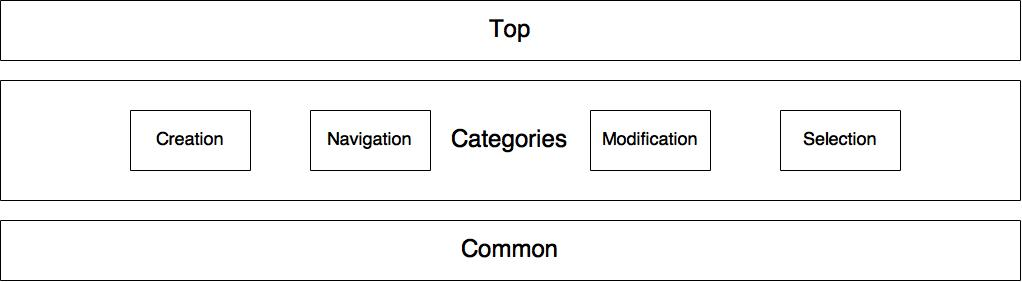
\includegraphics[scale=0.4]{./fig/BNFDiagram}
	\caption{This is the architecture of the Dictation Parser rules}
	\label{fig21}
\end{figure}

\subsection{Parser}
This section describes the parser of the Dictation Parser module. All layers are divided into tables; every table groups the commands of the layer.

\subsubsection{Top Layer}
\autoref{tab24} represents the commands of the Top layer.
\begin{table}[H]
	\centering
	\begin{tabular}{|p{8cm}|p{7cm}|}
		\hline
		\multicolumn{1}{|c|}{{\bf Rule}}                                                                                             & \multicolumn{1}{c|}{{\bf Description}} \\ \hline
		command: creationCommand | navigationCommand | selectionCommand | modificationCommand | deletionCommand | invocationCommand; & This is the main command               \\ \hline
	\end{tabular}
	\caption{This table represents the commands of the Top layer.}
	\label{tab24}
\end{table}

\subsubsection{Creation Layer}
\autoref{tab25} and \autoref{tab26} represents the commands of the Creation Layer. This layer handles all creation commands that the user dictates.
\begin{table}[H]
	\centering
	\begin{tabular}{|p{8cm}|p{7cm}|}
		\hline
		\multicolumn{1}{|c|}{{\bf Rule}} & \multicolumn{1}{c|}{{\bf Description}} \\ \hline
		creationCommand: creationVerb? (AN | A)? (createField | createMethod | createConstructor | createDataType | createBlock | createLoop) elementLocation?; & The main command of the Creation Layer \\ \hline
		creationVerb: CREATE | NEW | OPEN; & Creation verb                          \\ \hline
		createField: fieldModifier? fieldRef; & Creates a field                        \\ \hline
		createMethod: modifier? (METHOD | FUNCTION) namedElement ((THAT\_ACCEPTS | WITH) parametersList)? (returnsVars Element)?;                               & Creates a method                       \\ \hline
		createConstructor: modifier? CONSTRUCTOR ((THAT\_ACCEPTS | WITH) parametersList)?;                                                                      & Creates a constructor                  \\ \hline
		createDataType: modifier? (INNER)? dataType namedElement ((implementsVars | extendsVars) Element)?;                                                     & Creates a data type                    \\ \hline
		createBlock: BLOCK | createBlockStatement;                                                                                                              & Creates a block                        \\ \hline
	\end{tabular}
	\caption{This table represents the commands of the Creation layer.}
	\label{tab25}
\end{table}

\begin{table}[H]
	\centering
	\begin{tabular}{|p{8cm}|p{7cm}|}
		\hline
		\multicolumn{1}{|c|}{{\bf Rule}} & \multicolumn{1}{c|}{{\bf Description}} \\ \hline
		createBlockStatement: localVariableDeclaration | statement;                                                                                             & Creates a block of stattements         \\ \hline
		createLoop: createForEachLoop | createWhileLoop | createDoWhileLoop | createForLoop;                                                                    & Creates a loop                         \\ \hline
		createForEachLoop: FOR\_EACH Element IN Element command?;                                                                                               & Creates a foreach loop                 \\ \hline
		createWhileLoop: WHILE expression DO? command?;                                                                                                         & Creates a while loop                   \\ \hline
		createDoWhileLoop: DO command WHILE expression;                                                                                                         & Creates a do while loop                \\ \hline
		createForLoop: FOR Element (FROM (number | elementsElement))? (TO (number | elementsElement))? command?;                                                & Creates a for loop                     \\ \hline
	\end{tabular}
	\caption{This table represents the commands of the Creation layer.}
	\label{tab26}
\end{table}

\subsubsection{Navigation Layer}
\autoref{tab27} represents the commands of the Navigation Layer.  This layer handles all navigation commands that the user dictates.

\begin{table}[H]
	\centering
	\begin{tabular}{|p{8cm}|p{7cm}|}
		\hline
		\multicolumn{1}{|c|}{{\bf Rule}} & \multicolumn{1}{c|}{{\bf Description}} \\ \hline
		navigationCommand: navigationVerb (dataType | FIELD | METHOD)? Element | exitCommand; & Creates navigation command             \\ \hline
		navigationVerb: GO\_TO | WE\_ARE\_DONE\_WITH; & Navigation verb                        \\ \hline
		exitCommand: (EXIT | QUIT) (elementsElement | (dataType | FIELD | METHOD)? Element);  & Creates exit command                   \\ \hline
		exit: WE\_ARE\_DONE\_WITH | EXIT; & Variations of exit                     \\ \hline
	\end{tabular}
	\caption{This table represents the commands of the Navigation layer.}
	\label{tab27}
\end{table}

\subsubsection{Modification Layer}
\autoref{tab28} represents the commands of the Modification Layer. This layer handles all modification commands that the user dictates.

\begin{table}[H]
	\centering
	\begin{tabular}{|p{8cm}|p{7cm}|}
		\hline
		\multicolumn{1}{|c|}{{\bf Rule}}                 & \multicolumn{1}{c|}{{\bf Description}}                                 \\ \hline
		modificationCommand: modifyAccessLevel;          & Creates modification command                                           \\ \hline
		modifyAccessLevel: modificationVerb accessLevel; & Modifies the access level. For example, changes from private to public \\ \hline
		modificationVerb: MAKE\_IT | CHANGE\_IT;         & Modification verb                                                      \\ \hline
	\end{tabular}
	\caption{This table represents the commands of the Modification layer.}
	\label{tab28}
\end{table}

\subsubsection{Selection Layer}
\autoref{tab29} represents the commands of the Selection Layer.  This layer handles all selection commands that the user dictates.

\begin{table}[H]
	\centering
	\begin{tabular}{|p{8cm}|p{7cm}|}
		\hline
		\multicolumn{1}{|c|}{{\bf Rule}}             & \multicolumn{1}{c|}{{\bf Description}} \\ \hline
		selectionCommand: (NUMBER | OPTION)? number; & Creates selection command              \\ \hline
	\end{tabular}
	\caption{This table represents the commands of the Selection layer.}
	\label{tab29}
\end{table}

\subsubsection{Deletion Layer}
\autoref{tab30} represents the commands of the Deletion Layer.  This layer handles all deletion commands that the user dictates.

\begin{table}[H]
	\centering
	\begin{tabular}{|p{8cm}|p{7cm}|}
		\hline
		\multicolumn{1}{|c|}{{\bf Rule}}                             & \multicolumn{1}{c|}{{\bf Description}} \\ \hline
		deletionCommand: (DELETE | REMOVE) (line | elementsElement); & Creates deletion command               \\ \hline
	\end{tabular}
	\caption{This table represents the commands of the Deletion layer.}
	\label{tab30}
\end{table}

\subsubsection{Invocation Layer}
\autoref{tab31} represents the commands of the Invocation Layer.  This layer handles all invocation commands that the user dictates.

\begin{table}[H]
	\centering
	\begin{tabular}{|p{8cm}|p{7cm}|}
		\hline
		\multicolumn{1}{|c|}{{\bf Rule}}          & \multicolumn{1}{c|}{{\bf Description}} \\ \hline
		invocationCommand: CALL? elementsElement; & Creates invoke command                 \\ \hline
	\end{tabular}
	\caption{This table represents the commands of the Invocation layer.}
	\label{tab31}
\end{table}

\subsubsection{Common Layer}
\autoref{tab32} and \autoref{tab33} represent the commands of the Invocation Layer.  This layer handles all invocation commands that the user dictates.

\begin{table}[H]
	\centering
	\begin{tabular}{|p{8cm}|p{7cm}|}
		\hline
		\multicolumn{1}{|c|}{{\bf Rule}}                                                                                                                                                                                                                                                                                                                                                                                                      & \multicolumn{1}{c|}{{\bf Description}} \\ \hline
		fieldModifier: (FINAL | CONST)? modifier TRANSIENT? VOLATILE?; & Adds different modifications to a field. For example, final static public. \\ \hline
		variableModifier: (FINAL | CONST) | STATIC; & Adds final or static to a field. \\ \hline
		modifier: ABSTRACT? STATIC? accessLevel; & Adds abstract, static and access level. \\ \hline
		accessLevel: PRIVATE | PUBLIC | PROTECTED; & Adds access level. \\ \hline
		localVariableDeclaration: variableModifier* elementsName OF\_TYPE Element; & Declares a local variable. \\ \hline
		statement: expression | RETURN expression? | TRY CATCH? FINALLY? | THROW expression | SWITCH expression? | BREAK | CONTINUE | caseVars elementsElement; & Defines a statement. \\ \hline
		expression: primary | expression (plusVars plusVars | minusVars minusVars) | expression (equalsVars | isDifferentVars | lessThanEqualsVars | greaterThanEqualVars | greaterThanVars | lessThanVars | IS\_NOT | IS) expression | (plusVars | minusVars | plusVars plusVars | minusVars minusVars) expression | IF expression ((AND | OR) expression)* THEN command (ELSE command)? | expression (equalsVars | isDifferentVars | lessThanEqualsVars | greaterThanEqualVars | greaterThanVars | lessThanVars | IS\_NOT | IS) expression | NEW (expression | elementRef) | ASSIGN expression TO expression; & Defines an expression. \\ \hline
	\end{tabular}
	\caption{This table represents the commands of the Common layer.}
	\label{tab32}
\end{table}

\begin{table}[H]
	\centering
	\begin{tabular}{|p{8cm}|p{7cm}|}
		\hline
		\multicolumn{1}{|c|}{{\bf Rule}} & \multicolumn{1}{c|}{{\bf Description}} \\ \hline
		primary: OPEN\_PARENTHESES expression? | elementsElement | number; & Defines the most primitive expression. \\ \hline
		elementsElement: (elementRef OF)? elementRef; & Reference to an element of an element. For example, method of a class. \\ \hline
		elementLocation: locationRef (elementRef | line); & Reference to element location. \\ \hline
		fieldRef:,FIELD (elementsName? OF\_TYPE Element | OF\_TYPE Element namedElement | elementsName); & Reference to a field. \\ \hline
		elementRef: classRef | fieldRef | enumRef | interfaceRef | unspecifiedRef; & Reference to an element. \\ \hline
		classRef: CLASS Element; & Reference to a class. \\ \hline
		namedElement: reference? elementsName; & Reference to an element. \\ \hline
		elementsName: (Element AND)* Element; & Defines a set of elements. \\ \hline
		enumRef: ENUM Element; & Reference to an enum. \\ \hline
		interfaceRef: INTERFACE Element; & Reference to an interface. \\ \hline
		unspecifiedRef: Element; & Reference to an unspecified element. \\ \hline
		reference: NAMED | CALLED; & Different variations of references. \\ \hline
		locationRef: INSIDE | IN | AFTER | BEFORE | ABOVE | BELOW; & Defines variations of locations. \\ \hline
		parametersList: (parameter AND)* parameter; & Defines a list of parameters. \\ \hline
		parameter: elementsElement (OF\_TYPE Element)?; & Defines a parameter, \\ \hline
		dataType: CLASS | ENUM | INTERFACE; & Defines data types. \\ \hline
		line: LINE NUMBER? number; & Defines a line. For example, line number 6. \\ \hline
		number: Number | ZERO | ONE | TWO | THREE | FOUR | FIVE | SIX | SEVEN | EIGHT | NINE; & Defins numbers. \\ \hline
	\end{tabular}
	\caption{This table is the continuation of \autoref{tab32}.}
	\label{tab33}
\end{table}

\subsubsection{Forms of Expressions}
\autoref{tab34} and \autoref{tab35} represents the commands of the forms of expressions.

\begin{table}[H]
	\centering
	\begin{tabular}{|p{8cm}|p{7cm}|}
		\hline
		\multicolumn{1}{|c|}{{\bf Rule}} & \multicolumn{1}{c|}{{\bf Description}} \\ \hline
		returnsVars: THAT\_RETURNS | RETURNS | RETURN; & Defines different variations to pronounce "returns". \\ \hline
		implementsVars: IMPLEMENTS | IMPLEMENT | THAT\_IMPLEMENTS; & Defines different variations to pronounce "implements". \\ \hline
		extendsVars: EXTENDS | EXTEND | THAT\_EXTENDS; & Defines different variations to pronounce "extends". \\ \hline
		plusVars: PLUS | MATH\_PLUS; & Defines different variations to pronounce "plus". \\ \hline
		minusVars: MINUS | MATH\_MINUS; & Defines different variations to pronounce "minus". \\ \hline
		equalsVars: IS\_EQUAL\_TO | EQUAL\_TO | EQUALS\_TO | EQUALS | IS\_EQUALS; & Defines different variations to pronounce "equals". \\ \hline
		isDifferentVars: IS\_DIFFERENT\_FROM | DIFFERENT\_FROM; & Defines different variations to pronounce "is different". \\ \hline
		lessThanVars: LESS\_THAN | LESS\_THAN\_MATH | IS\_LESS\_THAN; & Defines different variations to pronounce "less than". \\ \hline
		lessThanEqualsVars: LESS\_THAN\_EQUAL | LESS\_THAN\_EQUAL\_MATH | LESS\_THAN\_EQUAL\_MATH\_SPACE; & Defines different variations to pronounce "less than equals". \\ \hline
	\end{tabular}
	\caption{This table represents the commands of the forms of expressions of different commands.}
	\label{tab34}
\end{table}

\begin{table}[H]
	\centering
	\begin{tabular}{|p{8cm}|p{7cm}|}
		\hline
		\multicolumn{1}{|c|}{{\bf Rule}} & \multicolumn{1}{c|}{{\bf Description}} \\ \hline
		greaterThanVars: GREATER\_THAN | GREATER\_THAN\_MATH | IS\_GREATER\_THAN; & Defines different variations to pronounce "greater than". \\ \hline
		greaterThanEqualVars: GREATER\_THAN\_EQUAL | GREATER\_THAN\_EQUAL\_MATH | GREATER\_THAN\_EQUAL\_MATH\_SPACE; & Defines different variations to pronounce "greater than equal". \\ \hline
		forEachVars: FOR\_EACH | FOR\_EACH\_SPACE; & Defines different variations to pronounce "for each". \\ \hline
		caseVars : CASE | IN\_CASE; & Defines different variations to pronounce "case". \\ \hline
	\end{tabular}
	\caption{This table is the continuation of \autoref{tab34}.}
	\label{tab35}
\end{table}

\subsection{Lexer}
This section describes the lexer of the Dictation Parser module. The lexer is built so it only has simple regular expressions and definitions.
\begin{itemize}
	\item METHOD: 'method';
	\item FUNCTION: 'function';
	\item CONSTRUCTOR: 'constructor';
	\item FIELD: 'field';
	\item BLOCK: 'block';
	\item INSIDE: 'inside';
	\item IN: 'in';
	\item AFTER: 'after';
	\item BEFORE: 'before';
	\item ABOVE: 'above';
	\item BELOW: 'below';
	\item INNER: 'inner';
	\item OF\_TYPE: 'of type';
	\item NEW: 'new';
	\item NAMED: 'named';
	\item CALLED: 'called';
	\item LINE: 'line';
	\item NUMBER: 'number';
	\item OPTION: 'option';
	\item AN: 'an';
	\item A: 'a';
	\item THAT\_ACCEPTS: 'that accepts';
	\item WITH: 'with';
	\item AND: 'and';
	\item OR: 'or';
	\item TO: 'to';
	\item FROM: 'from';
	\item GO\_TO: 'go to';
	\item EXIT: 'exit';
	\item QUIT: 'quit';
	\item WE\_ARE\_DONE\_WITH: 'we are done with';
	\item MAKE\_IT: 'make it';
	\item CHANGE\_IT: 'change it to';
	\item CREATE: 'create';
	\item OPEN: 'open';
	\item OPEN\_PARENTHESES: 'open parentheses';
	\item CALL: 'call';
	\item OF: 'of';
	\item PERIOD: 'period';
	\item PERIOD\_CHAR: '.';
	\item DELETE: 'delete';
	\item REMOVE: 'remove';
	\item ASSIGN: 'assign';
	\item PLUS: 'plus';
	\item MATH\_PLUS: '+';
	\item MINUS: 'minus';
	\item MATH\_MINUS: '-';
	\item IS: 'is';
	\item IS\_NOT: 'is not';
	\item IS\_EQUAL\_TO: 'is equal to';
	\item EQUAL\_TO: 'equal to';
	\item EQUALS\_TO: 'equals to';
	\item EQUALS: 'equals';
	\item IS\_EQUALS: 'is equals';
	\item IS\_DIFFERENT\_FROM: 'is different from';
	\item DIFFERENT\_FROM: 'different from';
	\item LESS\_THAN: 'less than';
	\item LESS\_THAN\_MATH: '<';
	\item IS\_LESS\_THAN: 'is less than';
	\item IS\_LESS\_THAN\_EQUAL: 'is less than equal';
	\item IS\_LESS\_THAN\_EQUALS: 'is less than equals';
	\item LESS\_THAN\_EQUAL: 'less than equal';
	\item LESS\_THAN\_EQUALS: 'less than equals';
	\item LESS\_THAN\_EQUAL\_MATH: '<=';
	\item LESS\_THAN\_EQUAL\_MATH\_SPACE: '< =';
	\item GREATER\_THAN: 'greater than';
	\item GREATER\_THAN\_MATH: '>';
	\item IS\_GREATER\_THAN: 'is greater than';
	\item GREATER\_THAN\_EQUAL: 'greater than equal';
	\item GREATER\_THAN\_EQUAL\_MATH: '>=';
	\item GREATER\_THAN\_EQUAL\_MATH\_SPACE: '> =';
	\item IF: 'if';
	\item THEN: 'then';
	\item ABSTRACT: 'abstract';
	\item ASSERT: 'assert';
	\item CATCH: 'catch';
	\item CLASS: 'class';
	\item CONST: 'const';
	\item DO: 'do';
	\item ELSE: 'else';
	\item ENUM: 'enum';
	\item EXTENDS: 'extends';
	\item EXTEND: 'extend';
	\item THAT\_EXTENDS: 'that extends';
	\item FINAL: 'final';
	\item FOR: 'for';
	\item IMPLEMENTS: 'implements';
	\item THAT\_IMPLEMENTS: 'that implements';
	\item IMPLEMENT: 'implement';
	\item INTERFACE: 'interface';
	\item PRIVATE: 'private';
	\item PROTECTED: 'protected';
	\item PUBLIC: 'public';
	\item STATIC: 'static';
	\item SUPER: 'super';
	\item THROW: 'throw';
	\item THROWS: 'throws';
	\item TRANSIENT: 'transient';
	\item TRY: 'try';
	\item VOID: 'void';
	\item VOLATILE: 'volatile';
	\item WHILE: 'while';
	\item FOR\_EACH: 'foreach';
	\item FOR\_EACH\_SPACE: 'for each';
	\item THAT\_RETURNS: 'that returns';
	\item RETURNS: 'returns';
	\item RETURN: 'return';
	\item SWITCH: 'switch';
	\item SYNCHRONIZED: 'synchronized';
	\item STRICTFP: 'strictfp';
	\item NATIVE: 'native';
	\item PACKAGE: 'package';
	\item IMPORT: 'import';
	\item INSTANCEOF: 'instanceof';
	\item FINALLY: 'finally';
	\item CONTINUE: 'continue';
	\item DEFAULT: 'default';
	\item BREAK: 'break';
	\item CASE: 'case';
	\item IN\_CASE: 'in case';
	\item ZERO: 'zero';
	\item ONE: 'one';
	\item TWO: 'two';
	\item THREE: 'three';
	\item FOUR: 'four';
	\item FIVE: 'five';
	\item SIX: 'six';
	\item SEVEN: 'seven';
	\item EIGHT: 'eight';
	\item NINE: 'nine';
	\item WS: [ \textbackslash t \textbackslash r \textbackslash n \textbackslash u000C]+ -> skip;
	\item Number: [0-9]+;
	\item Element: [a-zA-Z0-9\-]+;
\end{itemize}

\begin{figure}[H]
	\begin{lstlisting}
	for(int i = 0; i < n; i++)
	\end{lstlisting}
	\caption{A simple for loop}
	\label{fig20}
\end{figure}

\subsection{Grammar Testing} \label{subsection: Grammar Testing}
To test the grammar, we provide two programs and their transcripts. The first example is an implementation of a linked list and the second is an example of the Command design pattern. 
\subsubsection{LinkedList Example}
This is an implementation of the data structure linked list. \autoref{fig23}-\autoref{fig29} presents the program that implements Linked List. \autoref{itemize:LinkedList Dictation} lists the dictations that generate this program.
\begin{figure}[H]
	\begin{lstlisting}
	public class LinkedList implements Iterable {
		private Node head;
		private Node tail;
		private int size;
		
		public Iterator iterator(){
			return new LLIterator();
		}
		
		private class Node{
			public Object data;
			public Object next;
			
			public Node(Object data, Object next){
				this.next = next;
				this.data = data;
			}
			
			public Object getNext(){
				return next;
			}
			
			public Object getData(){
				return data;
			}
			
			public void setNext(Object next){
				this.next = next;
			}
		}
	\end{lstlisting}
	\caption{Implementation of Linked List in Java part 1}
	\label{fig23}
\end{figure}
\begin{figure}[H]
	\begin{lstlisting}
	private class LLIterator implements Iterator{
		private Node nextNode;
		private boolean removeOK;
		private int posToRemove;
		
		private LLIterator(){
			nextNode = head;
			removeOK = false;
			posToRemove = -1;
		}
		
		public boolean hasNext(){
			return nextNode != null;
		}
		
		public Object next(){
			assert hasNext();
			
			Object result = nextNode.getData();
			nextNode = nextNode.getNext();
			
			removeOK = true;
			posToRemove++;
			
			return result;
		}
	\end{lstlisting}
	\caption{Implementation of Linked List in Java part 2}
	\label{fig24}
\end{figure}
\begin{figure}[H]
	\begin{lstlisting}
			public void remove(){
				assert removeOK;
				removeOK = false;
				LinkedList.this.remove(posToRemove);
				posToRemove--;
				}
		}
			
		public void makeEmpty(){
			head = tail = null;
			size = 0;
		}
		
		public Object remove(int pos){
			assert pos >= 0 && pos < size;
			Object result;
			if( pos == 0 ){
				result = head.getData();
				
			head = head.getNext();
			if( size == 1 )
				tail = null;
			}
			else{    
				Node temp = head;
				for(int i = 1; i < pos; i++)
					temp = temp.getNext();
					
				result = temp.getNext().getData();
				temp.setNext( temp.getNext().getNext() );
				if( pos == size - 1)
					tail = temp;
			}
			size--;
			
			return result;
		}
		
		public Object get(int pos){
			assert pos >= 0 && pos < size;
			Object result;
			if( pos == size - 1 )
				result = tail.getData();
			else{
				Node temp = head;
				for(int i = 0; i < pos; i++)
					temp = temp.getNext();
					
				result = temp.getData();
			}
			
			return result;
		}
		
		public void insert(int pos, Object obj){
			assert pos >= 0 && pos <= size;
			if(pos == 0)
			addFirst(obj);
			
			else if( pos == size )
				add(obj);
			else{
				Node temp = head;
			for(int i = 1; i < pos; i++)
				temp = temp.getNext();
			
				Node newNode = new Node(obj, temp.getNext());
				temp.setNext( newNode );
				size++;
			}
		}
		
		public void add(Object obj){
			Node newNode = new Node(obj, null);
			if( size == 0 )
				head = newNode;
			else
				tail.setNext(newNode);
				
			tail = newNode;
			size++;
		}
		
		public void addFirst(Object obj){
			if(size == 0)
				add(obj);
			else{
				Node newNode = new Node(obj, head);
				head = newNode;
				size++;
			}
		}
		
		public String toString(){
			String result = "";
			Node temp = head;
			for(int i = 0; i < size; i++){
				result += temp.getData() + " ";
				temp = temp.getNext();
			}
			
			return result;
		}
	}
	\end{lstlisting}
	\caption{Implementation of Linked List in Java part 3}
	\label{fig25}
\end{figure}
\begin{figure}[H]
	\begin{lstlisting}
		public void remove(){
			assert removeOK;
			removeOK = false;
			LinkedList.this.remove(posToRemove);
			posToRemove--;
		}
	}
	
	public void makeEmpty(){
		head = tail = null;
		size = 0;
	}
	\end{lstlisting}
	\caption{Implementation of Linked List in Java part 4}
	\label{fig26}
\end{figure}
\begin{figure}[H]
	\begin{lstlisting}
	public Object remove(int pos){
		assert pos >= 0 && pos < size;
		Object result;
		if( pos == 0 ){
			result = head.getData();
			head = head.getNext();
			if( size == 1 )
				tail = null;
		}
		else{    
			Node temp = head;
			for(int i = 1; i < pos; i++)
				temp = temp.getNext();
				
			result = temp.getNext().getData();
			temp.setNext( temp.getNext().getNext() );
			if( pos == size - 1)
				tail = temp;
		}
		size--;
		return result;
	}
	\end{lstlisting}
	\caption{Implementation of Linked List in Java part 5}
	\label{fig27}
\end{figure}
\begin{figure}[H]
	\begin{lstlisting}
	public Object get(int pos){
		assert pos >= 0 && pos < size;
		Object result;
		if( pos == size - 1 )
			result = tail.getData();
		else{
			Node temp = head;
			for(int i = 0; i < pos; i++)
				temp = temp.getNext();
				
			result = temp.getData();
		}
		
		return result;
	}
	
	public void insert(int pos, Object obj){
		assert pos >= 0 && pos <= size;
		if(pos == 0)
			addFirst(obj);
		
		else if( pos == size )
			add(obj);
		else{
			Node temp = head;
			for(int i = 1; i < pos; i++)
				temp = temp.getNext();
			
			Node newNode = new Node(obj, temp.getNext());
			temp.setNext( newNode );
			size++;
		}
	}
	\end{lstlisting}
	\caption{Implementation of Linked List in Java part 6}
	\label{fig28}
\end{figure}
\begin{figure}[H]
	\begin{lstlisting}
		public void add(Object obj){
			Node newNode = new Node(obj, null);
			if( size == 0 )
				head = newNode;
			else
				tail.setNext(newNode);
				
			tail = newNode;
			size++;
		}
		
		public void addFirst(Object obj){
			if(size == 0)
				add(obj);
			else{
				Node newNode = new Node(obj, head);
				head = newNode;
				size++;
			}
		}
		
		public String toString(){
			String result = "";
			Node temp = head;
			for(int i = 0; i < size; i++){
				result += temp.getData() + " ";
				temp = temp.getNext();
			}
			
			return result;
		}
	}
	\end{lstlisting}
	\caption{Implementation of Linked List in Java part 7}
	\label{fig29}
\end{figure}
This is the list of the dictations that generates the program.
\begin{itemize} \label{itemize:LinkedList Dictation}
	\item Create class LinkedList that implements Iterable
	\item Create private field head of type Node
	\item Create private field tail of type Node
	\item Create private field size of type int
	\item Create method iterator that returns Iterator
	\item Return new LLIterator
	\item Exit method iterator
	\item Create inner class Node
	\item Create field data of type Object
	\item Make it public
	\item Create public field next of type Object
	\item Create constructor that accepts data of type Object and next of type Node
	\item Assign next to this.next
	\item Assign data to this.data
	\item Create method getNext that returns Object
	\item Return next
	\item Create method getData that returns Object
	\item Return data
	\item Create method setNext that accepts next of type object
	\item Assign next to this.next
	\item Exit class Node
	\item Create inner class LLIterator that implement Iterator
	\item Create a constructor
	\item Assign head to field nextNode	
	\item Assign false to field removeOK
	\item Assign -1 to field posToRemove
	\item Ceate method hasNext that returns boolean
	\item Return is nextNode different from null
	\item Ceate method next that return Object
	\item Assert hasNext
	\item Create result of type object and assign nextNode.getData to it
	\item Call nextNode.getNext and assign it to nextNode
	\item Assign true to removeOK
	\item Increase posToRemove
	\item Return result
	\item Create method remove
	\item Assert removeOK
	\item Assign false to removeOK
	\item Call LinkedList.this.remove that accepts posToRemove
	\item Decrease posToRemove
	\item Exit LLIterator
	\item Crete method makeEmpty
	\item Assign null to tail and head
	\item Assign zero to size
	\item Create method remove that accept pos of type int and returns Object
	\item Assert is pos more than 0 and pos less than size
	\item Create result of type Object
	\item If pos equal to 0 then
	\item Call head.getData and assign it to result
	\item Call head.getNext and assign it to head
	\item If size equal 1 then
	\item Assign null to tail
	\item Exit the if
	\item Else
	\item Create temp of type Node and assign head to it
	\item For i from 1 to pos
	\item Call temp.getNext and assign it to temp
	\item Exit the loop
	\item Call temp.getNext.getData and assign it to result
	\item Call temp.setNext that accepts temp.getNext.getNext
	\item If pos equal size minus 1 then
	\item Assign temp to tail
	\item Exit else
	\item Decrease size
	\item return result
	\item Create method get that accepts pos of type int and returns Object
	\item Assert is pos more or equal to 0 and less than size
	\item Create result of type Object
	\item If pos equal size minus 1 then
	\item Call tail.getData and assign it to result
	\item Else
	\item Create temp of type Node and assign head to it
	\item For i from 0 to pos
	\item Call temp.getNext and assign it to temp
	\item Exit for
	\item Call temp.getData and assign it to result
	\item Exit else
	\item Return result
	\item Create method insert that accepts pos of type int and obj of type Object
	\item Assert is pos more or equal to 0 and less than size
	\item If pos equal to 0 then
	\item Call addFirst that accepts obj
	\item Else if pos equal size then
	\item Call add that accepts obj
	\item Else
	\item Assign head to temp of type Node
	\item For i from 1 to pos
	\item Call temp.getNext and assign it to temp
	\item Exit the for loop
	\item Create new Node that accepts obj and temp.getNext and assign it to newNode of type Node
	\item Call temp.setNext that accept newNode
	\item Increase size
	\item Exit method insert
	\item Create method add that accepts obj of type Object
	\item Create new Node that accepts obj and null and assign it to newNode of type Node
	\item If size equal 0 then
	\item Assign newNode to head
	\item Else
	\item Call tail.setNext that accepts newNode
	\item Exit
	\item Assign newNode to tail
	\item Increase size
	\item Create method addFirst that accepts obj of type Object
	\item If size equal 0 then
	\item Call add that accepts obj
	\item Else
	\item Create new Node that accepts obj and head and assign it to newNode of type Node
	\item Assign newNode to head
	\item Increase size
	\item Create method toString that returns String
	\item Create result of type String and initialize it with an empty string
	\item Assign head to temp of type Node
	\item For i from 0 to size
	\item Result plus equal temp.getData plus space
	\item Call temp.getNext and assign it to temp
	\item Exit the loop
	\item Return result
\end{itemize}
\subsubsection{Car Builder Example}
This is an implementation of the Builder design pattern. We created a class of type Car that has properties and contains an inner class of type CarBuilder that has the functionality to create an instance of Car. In addition, it has main. \autoref{fig30}-\autoref{fig31} presents the program that implements Linked List. \autoref{itemize:Car Builder Dictation} lists the dictations that generate this program.
\begin{figure}[H]
	\begin{lstlisting}
	public class Car{
		private String _wheels;
		private String _engine;
		private String _body;
		
		private Car(String wheels, String engine, String body){
			if(body == null || engine == null || wheels == null)
				return;
			
			_wheels = wheels;
			_engine = engine;
			_body = body;
		}
		
		public static class CarBuilder{
			String Body;
			String Wheels;
			String Engine;
			
			public Car BuildCar(){
				if(Body != null && Wheels != null && Engine != null){
					return new Car(Wheels, Engine, Body);
				}
				
				return null;
			}
		}
	\end{lstlisting}
	\caption{Implementation of the design pattern Builder that creates a class of type Car part 1}
	\label{fig30}
\end{figure}
\begin{figure}[H]
	\begin{lstlisting}
		public static void main(String[] args){
			Car.CarBuilder carBuilder = new CarBuilder();
			carBuilder.Engine = "honda";
			carBuilder.Wheels = "4";
			carBuilder.Body = "private";
			Car car;
			car = carBuilder.BuildCar();
		}
	}
	\end{lstlisting}
	\caption{Implementation of the design pattern Builder that creates a class of type Car part 2}
	\label{fig31}
\end{figure}
This is the list of the dictations that generate the program.
\begin{itemize} \label{itemize:Car Builder Dictation}
	\item Create class car
	\item Create field wheel of type string
	\item Create field engine of type string
	\item Create field body of type string
	\item Create private constructor that accept wheels of type string engine of type string and body of type string
	\item If body equals null or engine equals null or wheels equals null then return	
	\item Assign wheels to field wheels
	\item Assign engine to field engine
	\item Assign body to field body
	\item Create inner class CarBuilder
	\item Create public field body of type string
	\item Create public field wheels of type string
	\item Create public field engine of type string
	\item Create method buildCar that returns Car
	\item If body different from null or wheels different from null or engine different from null then return new car that accepts wheels engine and body
	\item Return null
	\item Create main inside car
	\item Create new CarBuilder and assign it to carBuilder of type carBuilder
	\item Assign honda as string to carBuilder.engine
	\item Assign 4 as string to carBuilder.engine
	\item Assign private as string to carBuilder.engine
	\item Create car of type car
	\item Call carBuilder.BuildCar and assign it to car
\end{itemize}
\section{Implementation}
To implement the \textit{Dictation Parser}, we reviewed different applications such as: BNFC, BNF Parser Generator, BNF for Java, Antlr 4. We decided to use Antlr 4 because it can be integrated well in our solution, it is a popular and well-known tool and it is well known to other members of the team. The implementation of the \textit{Dictation Parser} is explained in details in \ref{section:BNF Parser}.